%! TEX root = ../root/raiz.tex
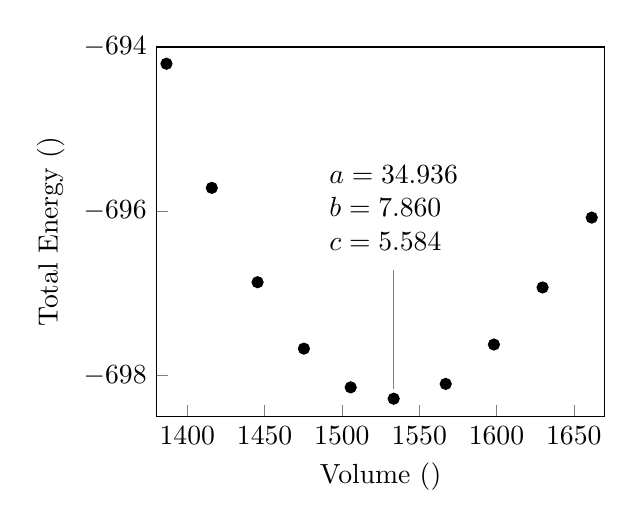
\begin{tikzpicture}
    \begin{axis}
        [
            width=.6\linewidth,
            legend pos={outer north east},
            legend style={draw=none},
            legend cell align=left,
            tick align=inside,
            tick pos=left,
            minor tick num=0,
            xlabel={Volume (\si{\cubic\angstrom})},
            xmin=1380,xmax=1670,
            xticklabel style={
                /pgf/number format/.cd,
                1000 sep={}
            },
            ylabel={Total Energy (\si{\electronvolt})},
            ymin=-698.5,ymax=-694.0
        ]
        \addplot [black, only marks, mark=*] table {
            1386.510000 -694.204090
            1415.850000 -695.715700
            1445.460000 -696.864600
            1475.420000 -697.673050
            1505.690000 -698.144720
            1533.490000 -698.283170
            1567.150000 -698.102660
            1598.330000 -697.623360
            1629.800000 -696.928260
            1661.600000 -696.077610
        }
        node [pin={[pin distance=10ex]90:\begin{tabular}{l}$a=\SI{34.936}{\angstrom}$\\$b=\SI{7.860}{\angstrom}$\\$c=\SI{5.584}{\angstrom}$\\\end{tabular}}] at (1533.490000, -698.283170) {};
    \end{axis}
\end{tikzpicture}
